% !TeX root = ../main.tex
% Add the above to each chapter to make compiling the PDF easier in some editors.

\chapter{Integration into existing Android App}\label{chapter:Integration into existing App}

The Existing app, already had some features related to the open source car driving simulator "Speed Dreams", before going deeper into theses functionalities, the present structure and Appearance is being highlighted.
First of all, a dark theme has been chosen for the design of the App. As can be seen in Figure \ref{fig:main_screen}, the main screen contains different tiles for each task. It is possible to choose the source of intended input, therefore the user decides between loading an existing image (Figure \ref{fig:load_image}), or hitting the camera icon to call a life-video feed of the back-facing camera. Depending on the input source chosen, the wanted functionalities are either applied one single time on a loaded image or multiple times per second on the life input, either way the outputs are printed onto the original images. Both features, named "Vehicle Detection" and "Lane Detection" are pretty much self explaining, but it should be mentioned that both methods were being trained by "Speed Dreams" data, meaning that the Lane detection is good for detecting lanes in the game, but might not be that brilliant in detecting real lanes, furthermore the vehicle detection recognizes only the back of a red car in the virtual rally course.
\begin{figure}[H]
	\minipage{0.25\textwidth}
	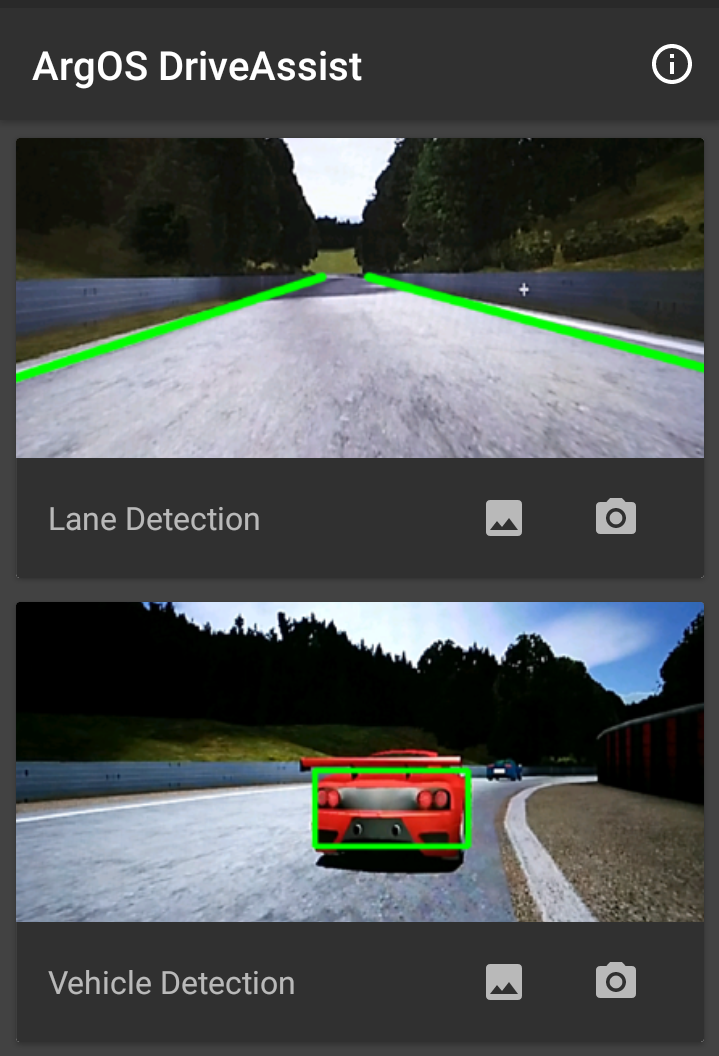
\includegraphics[height=5.2cm]{images/screenshot_main.png}
	\caption{Main screen}\label{fig:main_screen}
	\endminipage\hfill
	\minipage{0.25\textwidth}
	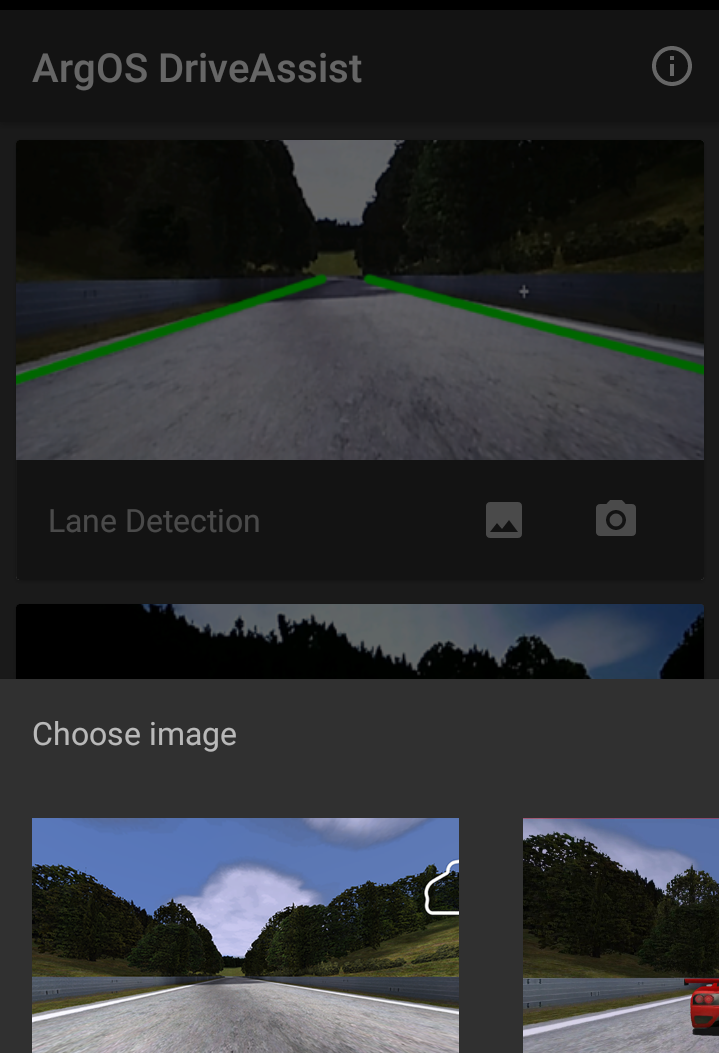
\includegraphics[height=5.2cm]{images/screenshot_load_image.png}
	\caption{Load\newline Image}\label{fig:load_image}
	\endminipage\hfill
	\minipage{0.25\textwidth}
	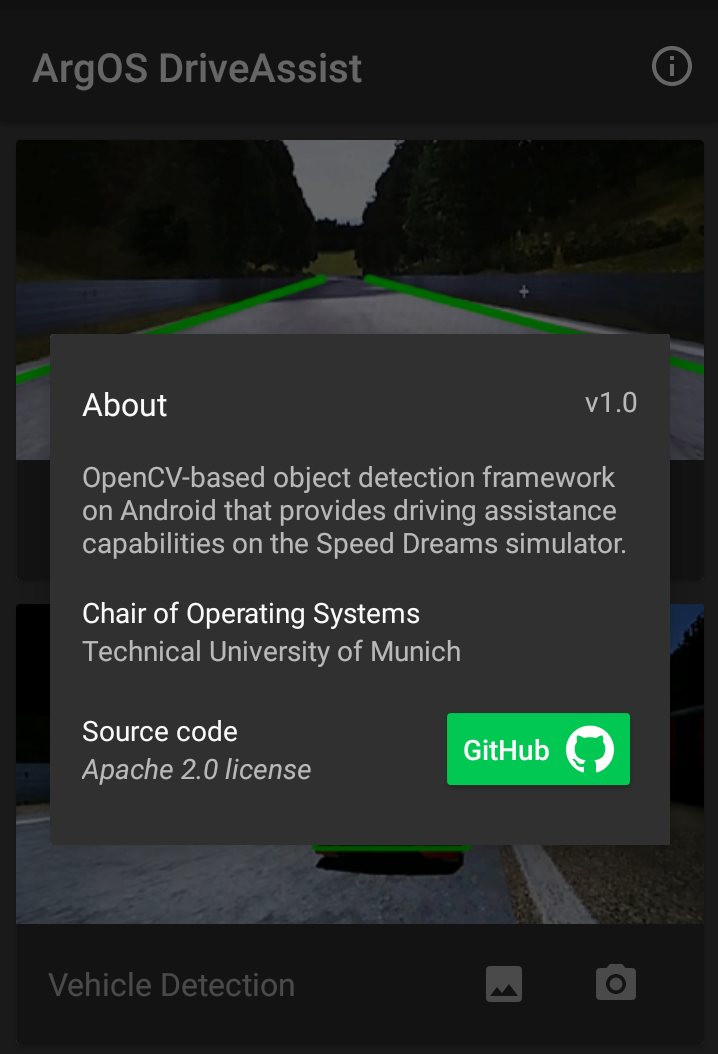
\includegraphics[height=5.2cm]{images/screenshot_about.png}
	\caption{About \newline infos}\label{fig:about}
	\endminipage\hfill
	\minipage{0.25\textwidth}
	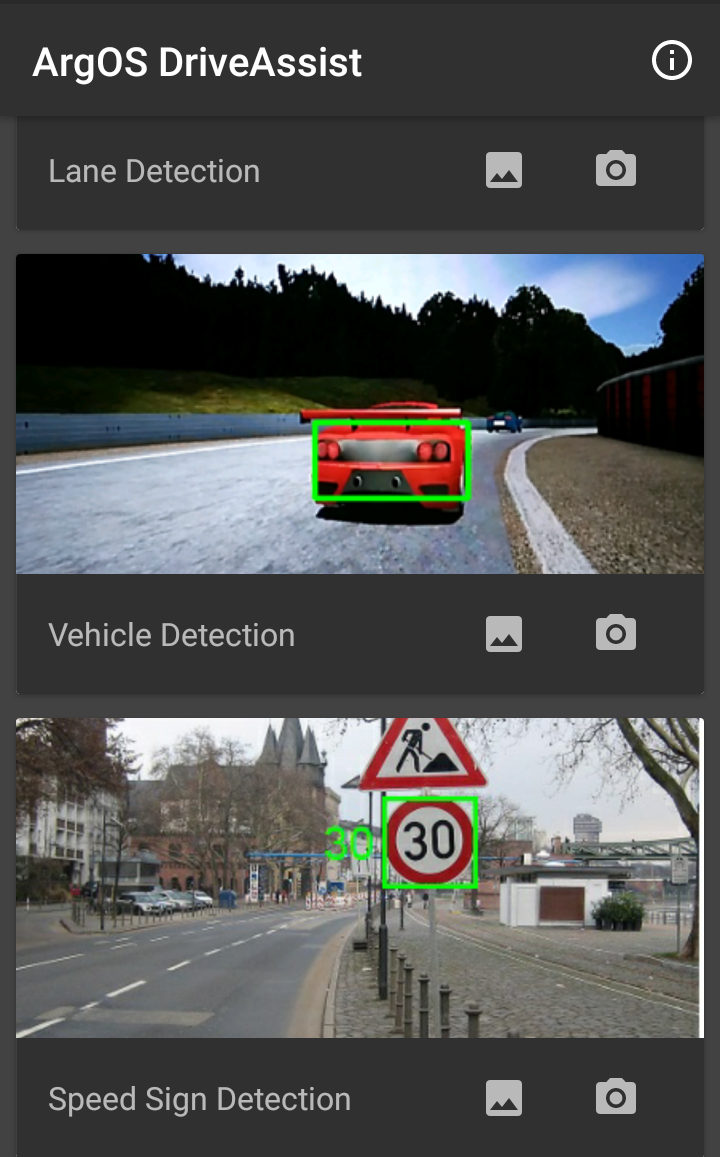
\includegraphics[height=5.2cm]{images/screenshot_new.png}
	\caption{New \newline tile}\label{fig:new}
	\endminipage
\end{figure}
To select the new functionalities, a new tile was added (Figure: \ref{fig:new}), having the same possibilities to choose from, as the already existing ones. As representative image, a picture with a speed sign was chosen and edited to look like how the actual detected image should. 







